%%%% Better Poster latex template example v1.0 (2019/04/04)
%%%% GNU General Public License v3.0
%%%% Rafael Bailo
%%%% https://github.com/rafaelbailo/betterposter-latex-template
%%%%
%%%% Original design from Mike Morrison
%%%% https://twitter.com/mikemorrison

\documentclass[fleqn,landscape]{betterposter}

% Draw some nice diagrams
\usepackage{tikz}
\usetikzlibrary{backgrounds}
\usetikzlibrary{arrows}
\tikzstyle{directed-top}=[->, very thick, white, line width=0.1em, tikzit draw=black]
\pgfkeys{/tikz/tikzit draw/.initial=0}
\pgfdeclarelayer{edgelayer}
\pgfdeclarelayer{nodelayer}
\pgfsetlayers{background, edgelayer, nodelayer, main}
\tikzstyle{none}=[inner sep=0mm]
%

%%%% Uncomment the following commands to customise the format

%% Setting the width of columns
% Left column
% \setlength{\leftbarwidth}{0.25\paperwidth}
% Right column
% \setlength{\rightbarwidth}{0.25\paperwidth}

%% Setting the column margins
% Horizontal margin
% \setlength{\columnmarginvertical}{0.05\paperheight}
% Vertical margin
% \setlength{\columnmarginhorizontal}{0.05\paperheight}
% Horizontal margin for the main column
% \setlength{\maincolumnmarginvertical}{0.15\paperheight}
% Vertical margin for the main column
% \setlength{\maincolumnmarginhorizontal}{0.15\paperheight}

%% Changing font sizes
% Text font
% \renewcommand{\fontsizestandard}{\fontsize{28}{35} \selectfont}
% Main column font
% \renewcommand{\fontsizemain}{\fontsize{28}{35} \selectfont}
% Title font
% \renewcommand{\fontsizetitle}{\fontsize{28}{35} \selectfont}
% Author font
% \renewcommand{\fontsizeauthor}{\fontsize{28}{35} \selectfont}
% Section font
% \renewcommand{\fontsizesection}{\fontsize{28}{35} \selectfont}

%% Changing font sizes for a specific text segment
% Place the text inside brackets:
% {\fontsize{28}{35} \selectfont Your text goes here}

%% Changing colours
% Background of side columns
% \renewcommand{\columnbackgroundcolor}{black}
% Font of side columns
% \renewcommand{\columnfontcolor}{gray}
% Background of main column
% \renewcommand{\maincolumnbackgroundcolor}{empirical}
% \renewcommand{\maincolumnbackgroundcolor}{theory}
% \renewcommand{\maincolumnbackgroundcolor}{methods}
% \renewcommand{\maincolumnbackgroundcolor}{intervention}
% Font of main column
% \renewcommand{\maincolumnfontcolor}{gray}

\begin{document}

\betterposter{
  %%%%%%%% MAIN COLUMN

  \maincolumn{
    %%%% Main space

    \textbf{Main finding} goes here,
    \\translated into \textbf{plain English}.
    \\\textbf{Emphasize} the important words.
  }{
    %%%% Bottom space

    %% QR code
    \begin{minipage}[t][-2em][b]{0.85\textwidth}
      \begin{minipage}{0.25\textwidth}
        \qrcode[nolinks, height=10cm]{https://arxiv.org/abs/2301.03545}
      \end{minipage}%
      \fontsizestandard
      \begin{minipage}[t][0.10\textheight][b]{0.24\textwidth}
        \begin{tikzpicture}[scale=3]
          \begin{pgfonlayer}{nodelayer}
            \node [style=none] (0) at (2, 0.5) {};
            \node [style=none] (1) at (0.5, 2) {};
            \node [style=none] (2) at (2, 0) {Get the paper here!};
          \end{pgfonlayer}
          \begin{pgfonlayer}{edgelayer}
            \draw [style=directed-top, in=0, out=90] (0.center) to (1.center);
          \end{pgfonlayer}
        \end{tikzpicture}
      \end{minipage}%
    \end{minipage}

  }

}{
  %%%%%%%% LEFT COLUMN

  \title{The Title}
  \vspace{-1em}
  \author{Mike Morrison and Rafael Bailo}
  \institution{Optional Institution Under Name}

  \section{Introduction}
  Here is an itemised list:
  \begin{itemize}
    \item The first item.
    \item The second item.
    \item The third item.
  \end{itemize}

  \section{A Diagram}
  Here is a diagram:
  \begin{center}
    % Linear regression
    % Author: Henri Menke
    % Retrieved from: http://www.texample.net/tikz/examples/linear-regression/
    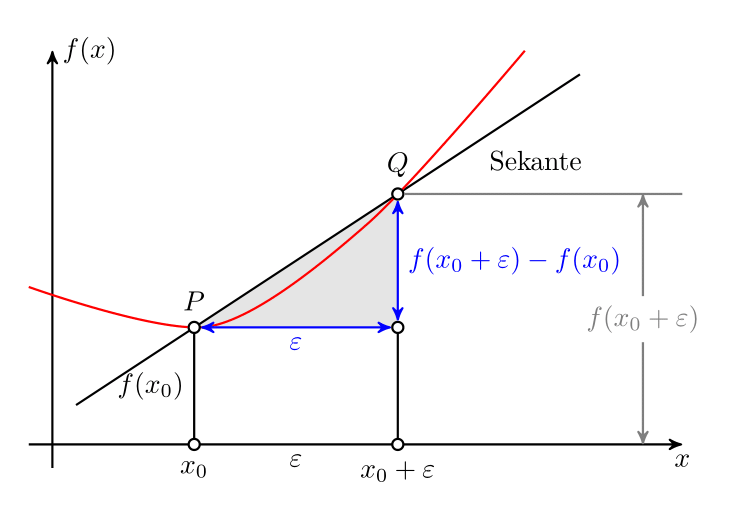
\includegraphics[width=\textwidth]{img/tikzexample1}
  \end{center}

  \section{Fundamental Theorem\\of Calculus}
  If \(f\) is continuous on the closed interval \([a,b]\) and \(F\) is the indefinite integral of \(f\) on \([a,b]\), then
  \begin{equation}
    \int_a^b f(x)\,\mathrm{d}x = F(b)-F(a).
  \end{equation}

  \section{Conclusion}
  This is a great poster format!

}{
  %%%%%%%% RIGHT COLUMN

  Here you can add \textbf{supplementary material}. For instance, a new diagram:
  \begin{center}
    % Commutative diagram with edges passing under/over
    % Author: Stefan Kottwitz, http://texblog.net/
    % Retrieved from: http://www.texample.net/tikz/examples/commutative-diagram/
    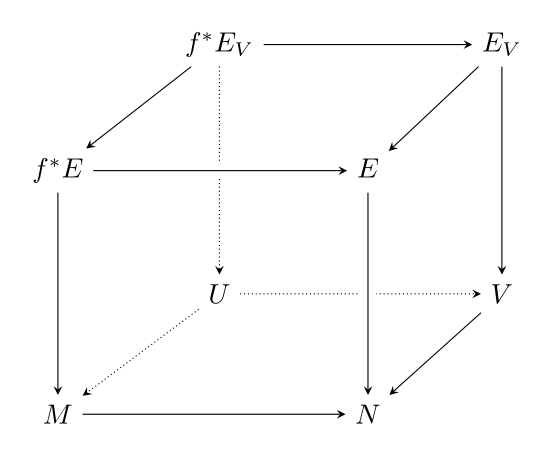
\includegraphics[width=\textwidth]{img/tikzexample2}
  \end{center}

  Some cute ducklings:
  \begin{center}
    % Picture of ducklings
    % Author: Magda Ehlers, https://www.pexels.com/@magda-ehlers-pexels
    % Retrieved from: https://www.pexels.com/photo/selective-focus-photo-of-flock-of-ducklings-perching-on-gray-concrete-pavement-1300355/
    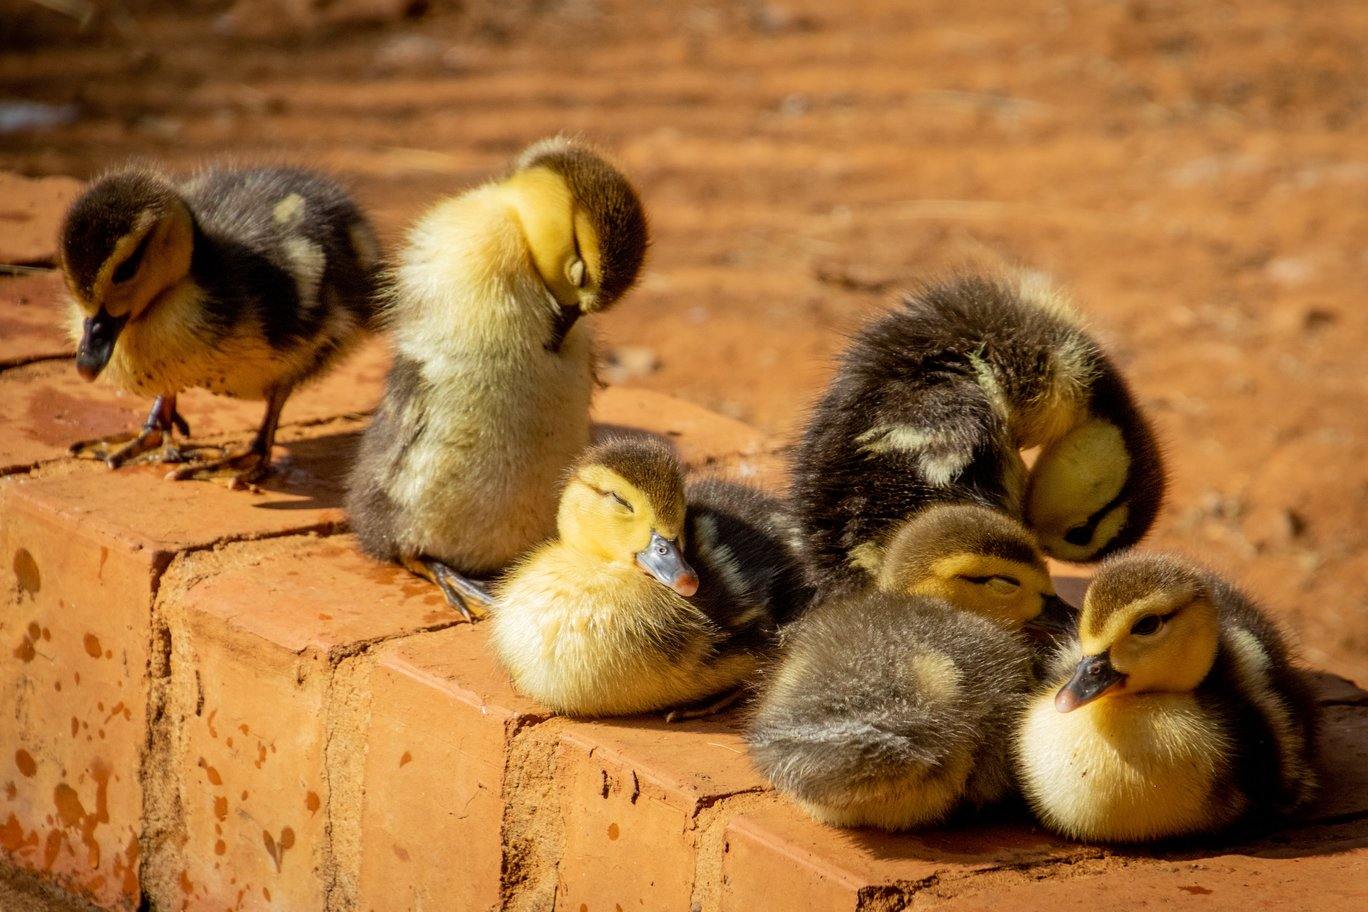
\includegraphics[width=\textwidth]{img/ducklings}
  \end{center}
}

\end{document}
